\documentclass[journal]{IEEEtran}

\usepackage{amsmath,amssymb}
\usepackage{graphicx}
\usepackage{booktabs}
\usepackage{array}
\usepackage{multirow}
\usepackage{cite}
\usepackage{url}
\usepackage{xspace}
\usepackage[hidelinks]{hyperref}

\graphicspath{{figures/}}
\newcommand{\xfull}{\textsc{XAI-Full}\xspace}
\newcommand{\pstatic}{p_{\mathrm{s}}}
\newcommand{\pdynamic}{p_{\mathrm{d}}}
\newcommand{\pfused}{p_{\mathrm{f}}}

\title{Auditable Adaptive Learning for Windows Malware Detection:\
Reliability-Aware Fusion, Explanation-Guided Sampling, and TreeSHAP Validation}

\author{Luu Van Doanh and Truong Ninh Thuan%
\thanks{The authors are with the VNU University of Engineering and Technology,
Vietnam National University, Hanoi, Vietnam.}%
}

\begin{document}
\maketitle

\begin{abstract}
Windows malware detection requires decisions from incomplete evidence while
expert labels remain scarce. Static scores provide early coverage, whereas
dynamic API prefixes supply complementary observations after execution; the
resulting models also require explanations that can be audited before they guide
data acquisition. We formulate these requirements as an auditable adaptive-
learning framework with three component-level research questions. First, a
control-inspired fusion rule maps disagreement between static and dynamic scores
to an adaptive weight and ablates proportional, integral, and derivative terms.
Second, a pool-based policy combines predictive uncertainty with TreeSHAP
directional entropy and attribution variance. Third, controlled deletion and
rank-stability tests assess whether TreeSHAP rankings track fitted-model
behavior. The components are evaluated on complementary, non-integrated
benchmarks: 1,922 paired MalBehavD-V1 samples for fusion and an identity-audited
2,000-sample, 2,381-feature EMBER subset for active learning and fidelity. On the
fusion development cohort, Adaptive P reduced false-positive rate from 12.45\%
to 11.16\% relative to fixed weighting (difference $-1.28$ percentage points;
95\% CI $[-2.47,-0.11]$) and improved Brier score, while integral and derivative
terms supplied no consistent incremental benefit. Across five outer folds and
five seeds, uncertainty plus directional entropy achieved the best ROC/AP
learning-curve areas; the full three-signal policy reached a predeclared
validation target with 492 labels, 92 (15.8\%) fewer than random acquisition.
Replacing the top 50 TreeSHAP-ranked features by training means reduced AUC by
0.306729, versus 0.000979 for equal-budget random replacement, with moderate
ranking stability. These results support component-wise evidence allocation and
model auditing for generic Windows malware; they do not constitute ransomware-
specific, external, or end-to-end validation.
\end{abstract}

\begin{IEEEkeywords}
active learning, explainable artificial intelligence, LightGBM, malware
detection, model auditing, PID control, score fusion, SHAP, TreeSHAP
\end{IEEEkeywords}

\section{Introduction}
\label{sec:introduction}

Machine-learning malware detectors operate under partial observability. A
portable executable (PE) can be inspected statically before execution, providing
immediate features from its headers, sections, imports, strings, and byte
statistics. This early evidence supports high-throughput screening, but packing,
obfuscation, source shift, and novel implementation choices can weaken learned
associations \cite{ucci2019survey,gibert2020rise,arp2022dos}. Dynamic analysis
reveals API calls and other behavior that a static representation may obscure,
but only after a monitored execution has produced enough events. It adds
collection cost, depends on the analysis environment, and can miss behavior that
does not manifest during observation \cite{sikorski2012practical,
sgandurra2016automated}. The operational question is therefore broader than
choosing one detector: a system must decide how to allocate heterogeneous
evidence as it becomes available.

The same allocation problem reappears during model maintenance. New labeled
software is expensive because an analyst must inspect only a small fraction of
an incoming pool. Uncertainty sampling prioritizes objects near a model boundary
\cite{cohn1996active,settles2009active}, yet it compresses the model's evidence
into a probability margin. Two samples can have the same output probability
while exhibiting different attribution structures: one may have uniformly weak
support, whereas another may combine strong positive and negative effects that
cancel. Explanation-derived structure can therefore supply a second view of
which labels may be informative. Once explanations influence sample selection,
however, they should not be accepted from a visualization alone. Their ranked
features must be tested against the fitted model, and their sensitivity to
training randomness and data partitions must be reported
\cite{warnecke2020evaluating,adebayo2018sanity}.

We organize these requirements as \emph{auditable evidence allocation under
partial observability}. The formulation has three connected stages. At the
decision stage, an early static score and sequential dynamic evidence must be
combined. At the adaptation stage, a restricted labeling budget must be assigned
to candidate samples. At the audit stage, the explanation mechanism used in
adaptation and model inspection must be subjected to controlled diagnostics. The
connection is conceptual and architectural: the same security-learning process
must allocate online evidence, offline labels, and trust in explanatory
artifacts. It does not imply that all components were evaluated on one dataset.

The first stage draws on proportional--integral--derivative (PID) control. In a
physical feedback loop, a PID controller transforms tracking error into an
actuation signal: the proportional term responds to present error, the integral
term accumulates persistent error, and the derivative term reacts to error
change \cite{astrom2001future}. We transfer this structure cautiously. Detector
disagreement replaces physical tracking error, and the controller output changes
the relative weight of static and dynamic scores. There is no physical plant or
closed-loop stability guarantee. The design is therefore \emph{control-inspired
score fusion}. This distinction is important because component ablation, rather
than the PID name, must determine whether temporal memory or a derivative term is
useful.

The latest paired evidence changes the scientific conclusion. On 1,922
MalBehavD-V1 samples with static metadata and ordered API events, a proportional
adaptive rule reduced false-positive rate (FPR) and Brier score relative to
validation-selected fixed weighting. A full PID rule obtained ranking
performance comparable to logistic stacking and a lower FPR at its selected
operating point, but it incurred a small true-positive-rate trade-off. More
importantly, PI and PID did not improve consistently over P within the examined
1--20-event horizon. We report this negative result directly and interpret it as
evidence-driven simplification: current disagreement is useful in this cohort,
whereas accumulated and derivative disagreement have not yet earned additional
complexity.

The adaptation and audit stages are evaluated on a separate, identity-audited
subset of EMBER \cite{anderson2018ember}. We combine predictive uncertainty with
two summaries of signed TreeSHAP contributions: directional entropy, which
measures the balance between positive and negative attribution mass, and
attribution variance across coordinates. Five acquisition policies are compared
under matched initial sets, pools, budgets, and outer folds. We then evaluate
TreeSHAP separately over 25 fitted models by replacing sample-specific
top-$|\mathrm{SHAP}|$ coordinates with training-derived mean or median values and
comparing the result with equal-budget random masks. Spearman and Jaccard
agreement distinguish seed sensitivity from fold sensitivity.

This component-wise design answers three research questions:

\begin{itemize}
    \item \textbf{RQ1---adaptive fusion:} On paired event-indexed static and
    dynamic evidence, how do P, PI, and PID fusion compare with average,
    max-risk, fixed weighting, and learned logistic stacking in discrimination,
    calibration, and operating-point trade-offs?
    \item \textbf{RQ2---label allocation:} Under matched training-label budgets,
    do directional entropy and SHAP variance add useful acquisition information
    beyond random and uncertainty-only selection?
    \item \textbf{RQ3---explanation audit:} Under training-derived mean and
    median replacement, do top-$|\mathrm{TreeSHAP}|$ coordinates affect fitted-
    model ranking more than equal-budget random coordinates, and how stable are
    the rankings across model seeds and data folds?
\end{itemize}

The study makes four contributions.

\begin{itemize}
    \item We formulate one auditable evidence-allocation problem that connects
    sequential decision fusion, budgeted model adaptation, and explanation
    verification while keeping their empirical estimands separate.
    \item We provide a paired comparison of simple and learned fusion rules on
    1,922 samples. Adaptive P improves FPR by 1.28 percentage points and Brier by
    0.00306 relative to fixed weighting, with paired-bootstrap intervals that
    exclude zero. The ablation also shows that I and D do not provide stable
    incremental value in the measured horizon.
    \item We evaluate explanation-guided active learning with five outer folds
    and five seeds. $U+H$ leads ROC/AP area under the learning curve (AULC),
    $U+V$ reaches the validation target with the fewest labels, and \xfull
    uses 92 fewer training labels than Random. No policy dominates every
    criterion.
    \item We test TreeSHAP rankings with controlled mean/median deletion and
    stability analysis. Top-ranked deletion produces substantially larger AUC
    decreases than random deletion, while moderate cross-model agreement exposes
    dependence on the fitted cohort.
\end{itemize}

The scope is deliberately narrower than a deployment claim. MalBehavD-V1 is
used for fusion; EMBER is used for active learning and fidelity. Their metrics
are not merged, and no active-learning--fusion interaction is claimed. Both
datasets have generic benign/malware labels, so the study does not establish
ransomware-specific or zero-day detection. The fusion comparison is development
evidence obtained after the original confirmatory analysis on the same cohort;
the active-learning and fidelity results are confirmatory under the retained
protocol. These evidence levels are visible in the tables and discussion.

The remainder of the paper is organized as follows.
Section~\ref{sec:related} reviews static/dynamic detection, score fusion, active
learning, and explanation validation. Section~\ref{sec:problem} states the
unified problem and claim boundaries. Section~\ref{sec:method} describes the
fusion, acquisition, and audit methods. Section~\ref{sec:protocol} separates the
two benchmark protocols and evidence tiers. Section~\ref{sec:results} reports
results by research question. Sections~\ref{sec:discussion} and
\ref{sec:threats} interpret the findings and threats to validity, and
Section~\ref{sec:conclusion} concludes.

\section{Related Work}
\label{sec:related}

\subsection{Static and Dynamic Windows Malware Detection}

Static malware analysis derives evidence without running a suspect object.
Learned detectors have used engineered binary attributes
\cite{saxe2015deep}, complete byte streams \cite{raff2018malware}, and documented
PE representations such as EMBER \cite{anderson2018ember}. SOREL-20M expanded
the scale of static PE research and supplied richer metadata
\cite{harang2020sorel}. Gradient-boosted trees remain effective on heterogeneous
tables containing histograms, strings, imports, sections, and header fields
\cite{ke2017lightgbm}. Their principal operational benefit is early scoring, but
static associations can be changed through packing, obfuscation, build-tool
variation, and distribution shift \cite{ucci2019survey,gibert2020rise}.

Dynamic analysis instead observes execution. API calls, file and registry
operations, process creation, and network activity can expose behavior absent
from a static vector \cite{sikorski2012practical,sgandurra2016automated}. The
evidence is conditional on the sandbox, inputs, run duration, and path reached by
the program. Delayed or environment-aware behavior can remain unobserved, while
longer collection increases resource cost. Work on ransomware illustrates the
value of behavior-centric analysis \cite{kharraz2015cutting,bacci2021ransomware},
but the present datasets contain generic malware labels. Those studies motivate
the analysis modes; they do not transfer ransomware semantics to our labels.

Hybrid systems commonly concatenate features, combine decisions, or fuse
scores. A concatenated model assumes that all modalities are available at once,
whereas sequential monitoring produces dynamic prefixes over time. Fixed score
averaging is transparent but cannot respond to sample-specific disagreement.
Learned stacking can capture a calibrated relation between channels, but it
requires a representative development cohort and can obscure how the weight
changes as evidence arrives. Meaningful evaluation must compare adaptive rules
with simple average, max-risk, fixed weighting, and a learned stacker using the
same paired samples and operating-point procedure.

\subsection{From Physical PID Control to Score Fusion}

PID control is a foundational feedback mechanism. Given reference $r(t)$,
measured output $y(t)$, and tracking error $e(t)=r(t)-y(t)$, proportional action
responds to present error, integral action addresses persistent accumulated
error, and derivative action anticipates rapid error change
\cite{astrom2001future}. These roles are meaningful in a physical loop with a
plant, time scale, actuation, and stability analysis.

Mapping PID structure to classifier fusion requires narrower language. Two
detector outputs are measurements, not a reference and controlled state.
Changing their weight does not alter the program being observed or close a
physical loop. In our formulation, static--dynamic disagreement is a surrogate
error and the controller output is a bounded mixture weight. The P/I/D terms
then provide hypotheses about useful memory: P reacts to current disagreement,
I represents persistent disagreement across prefixes, and D represents a change
in disagreement. No stability guarantee follows from this analogy. Validation
and component ablation decide whether any term improves prediction.

This framing addresses a common methodological gap. A controller name can make a
fusion rule appear inherently adaptive, even when each sample provides one
observation or the derivative rarely changes a decision. We retain P/PI/PID as
nested, testable models and report a negative I/D result. The contribution is
therefore an auditable translation and empirical simplification of a
control-inspired rule, rather than a claim that classical control theory proves
malware-classification performance.

\subsection{Active Learning and Batch Acquisition}

Pool-based active learning alternates model fitting, query selection, oracle
annotation, and retraining. Uncertainty sampling is widely used because it is
simple and model compatible \cite{cohn1996active,settles2009active}. In batch
settings, however, the highest-scoring samples can be redundant. Core-set
acquisition emphasizes representation coverage \cite{sener2018active}; ensemble
methods use predictive disagreement \cite{beluch2018power}; BatchBALD uses joint
mutual information \cite{kirsch2019batchbald}; and BADGE clusters uncertain
gradient embeddings \cite{ash2020deep}.

These methods are not equally portable to boosted trees. BatchBALD and BADGE
were designed around Bayesian or differentiable deep models, although their
principles motivate tree-compatible diversity and committee baselines. Our
measured policies include random sampling, uncertainty, two explanation-signal
ablations, and a three-signal combination. They do not include uncertainty plus
k-center diversity or a calibrated committee. We consequently test whether the
specific TreeSHAP summaries add value to the retained baselines, without claiming
general dominance over active learning.

Explanations may enter active learning as annotator-facing context or as an
algorithmic ranking signal. Explainable active learning has studied how local
explanations affect annotator experience \cite{ghai2021explainable}. Our use is
algorithmic: signed TreeSHAP summaries are computed before annotation and enter
the acquisition score. A balanced or dispersed attribution vector is not equal
to expected information gain; it is a falsifiable heuristic evaluated through
matched learning curves, target attainment, low-FPR summaries, and computation.

\subsection{Attribution and Explanation Validation}

LIME estimates a local surrogate \cite{ribeiro2016why}; SHAP unifies additive
feature attribution through Shapley values \cite{lundberg2017unified}; and
TreeSHAP specializes the calculation to tree ensembles
\cite{lundberg2020local}. Explanations can still be insensitive to model
parameters, manipulated, or misread as causal mechanisms
\cite{adebayo2018sanity,slack2020fooling}. Security inputs add domain constraints
and adversarial considerations \cite{warnecke2020evaluating}.

Deletion tests ask whether changing highly ranked coordinates alters model
output. Their conclusion depends on the intervention: independent replacement
can move a vector off the data manifold, and a large effect can reflect
perturbation magnitude as well as ranking quality
\cite{hooker2019benchmark,yeh2019infidelity}. Training-derived mean and median
baselines avoid assuming that zero is a semantically neutral PE value, but they
do not guarantee an executable-valid binary. Equal-count random masks control
the number of replaced coordinates, though they may select features unused by a
tree ensemble. Rank stability offers a complementary view by testing sensitivity
to model seeds and data folds.

\begin{table*}[t]
\centering
\caption{Positioning of the three components. “Open comparison” identifies an
evidence gate rather than a completed experiment.}
\label{tab:related}
\scriptsize
\setlength{\tabcolsep}{2.5pt}
\begin{tabular}{p{2.8cm}p{3.4cm}p{2.8cm}p{2.8cm}p{3.2cm}}
\toprule
Area & Representative approach & Strength & Limitation relevant here & Role in this study \\
\midrule
Static detection & EMBER/boosted trees \cite{anderson2018ember,ke2017lightgbm} & Early, scalable PE scoring & Static distribution shift and manipulation & AL/fidelity benchmark and static fusion channel \\
Dynamic detection & Sandbox/API behavior \cite{sgandurra2016automated} & Observes executed behavior & Environment and observation dependence & Event-indexed fusion channel \\
Fusion & Average/fixed/learned stacking & Transparent or data-adaptive combination & Fixed rules ignore disagreement; stacking can hide sequential behavior & Measured baselines for P/PI/PID \\
PID control & P/I/D feedback \cite{astrom2001future} & Interpretable current, accumulated, and rate terms & Classifier fusion has no physical plant or stability guarantee & Control-inspired nested ablation \\
Active learning & Uncertainty \cite{cohn1996active} & Simple and strong & Margin omits evidence structure & Measured baseline \\
Batch diversity & Core-set/committee \cite{sener2018active,beluch2018power} & Reduces redundancy or measures disagreement & Absent from retained artifact & Open comparison \\
Explanation guidance & Explainable AL \cite{ghai2021explainable} & Adds model rationale to selection/annotation & Explanation signal need not equal information gain & TreeSHAP summaries enter query score \\
XAI evaluation & Sanity/deletion tests \cite{adebayo2018sanity,hooker2019benchmark} & Tests model sensitivity & Intervention may be off-manifold & Mean/median deletion plus stability \\
\bottomrule
\end{tabular}
\end{table*}

Our novelty claim is correspondingly specific. We do not claim that static--
dynamic fusion, PID structure, active learning, or SHAP is individually new. We
contribute a scoped evidence-allocation formulation, a paired P/PI/PID fusion
ablation that supports simplification, a signed-mass TreeSHAP acquisition family,
and quantitative validation of the attribution ranking. The component-wise
protocol makes clear which links are empirically measured and which remain an
integration hypothesis.

\section{Unified Problem Formulation}
\label{sec:problem}

\subsection{Evidence Allocation under Partial Observability}

Let $i$ index a PE sample with binary label $y_i\in\{0,1\}$, where one denotes
generic malware. Static representation $x_i^{\mathrm{s}}$ is available before
execution and produces score $p_i^{\mathrm{s}}$. A monitored run produces an
ordered dynamic sequence
$z_i=(z_{i1},\ldots,z_{iT_i})$. At prefix $k$, dynamic model $g$ produces
$p_{ik}^{\mathrm{d}}=g(z_{i1:k})$. The online task is to map the available
evidence to a fused score
\begin{equation}
p_{ik}^{\mathrm{f}}=
F\!\left(p_i^{\mathrm{s}},p_{i1:k}^{\mathrm{d}};\theta_F\right),
\label{eq:online-object}
\end{equation}
and a decision at a validation-selected threshold. Because $k$ counts API
events, it is an observation index rather than elapsed seconds.

The development task has a different resource constraint. Given labeled set
$\mathcal{L}_r$, unlabeled pool $\mathcal{U}_r$, and batch budget $b$, model
$f_r$ ranks pool samples with acquisition function $Q_r$. The oracle reveals
labels only for selected batch $\mathcal{B}_r$:
\begin{equation}
\mathcal{B}_r=\operatorname*{arg\,top}_{\substack{
\mathcal{B}\subset\mathcal{U}_r\\|\mathcal{B}|=b}}
\sum_{x\in\mathcal{B}}Q_r(x),
\qquad
\mathcal{L}_{r+1}=\mathcal{L}_r\cup\mathcal{B}_r.
\label{eq:batch-object}
\end{equation}
The retained experiment uses a pointwise top-$b$ rule; it does not optimize
joint diversity.

The audit task operates on a fixed fitted model and explanation
$\boldsymbol{\phi}_i$. It tests whether coordinates ranked highly by
$|\boldsymbol{\phi}_i|$ produce greater model-performance degradation under a
specified replacement intervention than equal-count random coordinates. It also
measures ranking agreement across fitted models. This task estimates relative
model reliance and sensitivity, not causal behavior of the executable.

These three tasks share an allocation principle but not one objective function.
Online fusion allocates weight between evidence channels; active learning
allocates labeling budget; explanation audit allocates confidence to a ranked
attribution. Reporting one metric as proof of all three would conflate distinct
estimands. We therefore use one architecture and three RQs, with separate data
and evaluation units.

\subsection{Fusion Estimands}

Fusion is assessed along three axes. ROC--AUC and average precision (AP) measure
ranking. The Brier score
\begin{equation}
\mathrm{Brier}=\frac{1}{n}\sum_{i=1}^{n}(p_i-y_i)^2
\label{eq:brier}
\end{equation}
measures squared probabilistic error. FPR and TPR measure decisions at thresholds
selected using validation data. An FPR comparison is interpreted together with
TPR because two independently chosen thresholds need not correspond to the same
operating point.

Paired differences use identical test rows. For Adaptive P versus Fixed, the
primary operating-point effects are
$\Delta\mathrm{FPR}$, $\Delta\mathrm{TPR}$, and
$\Delta\mathrm{Brier}$. For PID versus learned stacking, the report additionally
uses $\Delta\mathrm{AUC}$. Bootstrap intervals quantify paired uncertainty over
the retained cohort. The post-confirmatory fusion development used this same
cohort; its intervals describe resampling uncertainty, not external
confirmation.

\subsection{Learning-Curve Estimands}

Every active-learning run produces ROC--AUC and AP at budgets
$B\in\{200,300,\ldots,1200\}$. For metric $m(B)$, normalized area under the
learning curve is
\begin{equation}
\mathrm{AULC}(m)=\frac{1}{B_{\max}-B_{\min}}
\int_{B_{\min}}^{B_{\max}}m(B)\,dB,
\label{eq:aulc}
\end{equation}
computed by trapezoidal integration over measured budgets. This quantity rewards
useful models earlier in the acquisition process. Endpoint comparison is less
informative because every policy eventually receives the same full pool.

A full-pool reference model defines a fold-specific validation target
\begin{equation}
t_{\mathrm{fold}}=0.5+0.95\left(
\mathrm{AUC}^{\mathrm{full}}_{\mathrm{val}}-0.5\right).
\label{eq:target}
\end{equation}
Labels-to-target is the first training budget that reaches this value. It counts
queried training labels; the validation labels, original retained labels, and
full-pool reference are additional experimental resources. Low-FPR summaries
include normalized partial AUC up to FPR 5\% and TPR-AULC at FPR caps of 1\% and
5\%. These are cohort metrics, not estimates for operational FPR near
$10^{-3}$ or below.

\subsection{Explanation Object and Intervention}

For a fitted tree model and sample $x_i\in\mathbb{R}^d$, let
$\boldsymbol{\phi}_i=(\phi_{i1},\ldots,\phi_{id})$ denote signed TreeSHAP
contributions and $\phi_{i0}$ the bias. Native TreeSHAP is verified on the raw
score scale:
\begin{equation}
f_{\mathrm{raw}}(x_i)=\phi_{i0}+\sum_{j=1}^{d}\phi_{ij}.
\label{eq:additivity}
\end{equation}
This identity checks numerical reconstruction; it does not verify feature
semantics or causal correctness.

For deletion budget $k$, sample-specific mask $M_i^{(k)}$ replaces selected
coordinates with training-derived baseline $b_j$:
\begin{equation}
\widetilde{x}_{ij}=\begin{cases}
b_j,&j\in M_i^{(k)},\\
x_{ij},&\text{otherwise}.
\end{cases}
\label{eq:mask}
\end{equation}
The top mask contains the $k$ largest $|\phi_{ij}|$ values; the control contains
$k$ uniformly sampled coordinates. $b_j$ is the training-column mean or median.
The comparison estimates fitted-model sensitivity under two feature-space
interventions. A modified vector need not correspond to a buildable or
executable PE file.

\subsection{Security and Claim Boundaries}

The labels in both benchmarks denote generic benign/malware status. Neither
dataset establishes ransomware ground truth. The EMBER folds are random row
folds, not temporal or family-disjoint splits. MalBehavD-V1 dynamic sequences are
event-indexed, not wall-clock traces, and source differences may correlate with
class. The study excludes a white-box adversary who manipulates features, pool
membership, or the oracle against the complete pipeline.

The unified architecture is consequently a research framework. The fusion
component is evaluated on MalBehavD-V1; active learning and fidelity are
evaluated on EMBER. There is no measured interaction between adaptive fusion and
active learning, no end-to-end latency, and no common cohort supporting a joint
performance metric. These boundaries determine the wording of the abstract,
results, and conclusion.

\section{Methodology}
\label{sec:method}

\subsection{Decision--Adaptation--Audit Architecture}

Figure~\ref{fig:architecture} presents the unified flow. The online decision path
computes a static score and, when behavioral evidence is available, updates a
dynamic score at ordered event prefixes. A fusion rule returns a final score.
The offline adaptation path trains a static model, ranks the remaining pool, asks
an oracle for a restricted label batch, and retrains. The audit path freezes a
model and tests the attribution ranking through controlled deletion and
cross-model stability.

\begin{figure*}[t]
\centering
\fbox{\begin{minipage}{0.96\textwidth}
\centering
\textbf{Online decision allocation (MalBehavD-V1)}\par\smallskip
PE metadata $\rightarrow \pstatic$
$\quad\parallel\quad$
ordered API prefixes $z_{1:k}\rightarrow p_{\mathrm{d},k}$
$\rightarrow$ validation-locked Average/Fixed/Stacking/P/PI/PID
$\rightarrow \pfused$ and decision
\par\medskip\hrule\medskip
\textbf{Offline label allocation (EMBER)}\par\smallskip
$\mathcal{L}_r\rightarrow$ LightGBM $\rightarrow$
pool probability and TreeSHAP $\rightarrow U,H,V\rightarrow Q_r$
$\rightarrow$ oracle batch $\rightarrow\mathcal{L}_{r+1}$
\par\medskip\hrule\medskip
\textbf{Explanation audit (EMBER)}\par\smallskip
fixed LightGBM $\rightarrow$ TreeSHAP ranking $\rightarrow$
top-$k$/random mean--median replacement $\rightarrow$
AUC degradation and seed/fold stability
\end{minipage}}
\caption{One auditable evidence-allocation formulation with component-wise
evaluation. Solid flows show the measured components. The horizontal boundaries
mark distinct benchmarks; they are not a single end-to-end experiment.}
\label{fig:architecture}
\end{figure*}

TreeSHAP has two offline roles. It supplies local summaries to the acquisition
function and a ranking to the audit experiment. These uses share a fitted
explanation method, but their estimands differ: acquisition asks which object to
label, while deletion asks whether a ranked coordinate set influences model
behavior under a specific intervention. A positive deletion result does not
prove that SHAP causes the active-learning improvement.

\subsection{Static Learner and TreeSHAP}

LightGBM represents a raw score as an additive tree ensemble
\begin{equation}
F(x)=\sum_{m=1}^{M}\eta h_m(x),
\label{eq:lgbm}
\end{equation}
where $h_m$ is a decision tree, $M$ is the number of boosting rounds, and $\eta$
is the learning rate \cite{ke2017lightgbm}. Its histogram-based learner handles
heterogeneous PE attributes without forcing a common feature unit. The binary
score follows from the logistic link.

Native TreeSHAP returns one signed contribution per feature and a separate bias
\cite{lundberg2020local}. Equation~(\ref{eq:additivity}) is checked before using
an explanation. The bias is excluded from feature ranking, directional entropy,
variance, and deletion budgets. Including it as a coordinate would confound the
model base rate with an observed PE feature.

\subsection{Control-Inspired Reliability-Aware Fusion}

\subsubsection{Translation from classical PID}

Classical discrete PID maps tracking error to an actuation signal. Here, the
available surrogate is detector disagreement at event prefix $k$:
\begin{equation}
e_{ik}=p_i^{\mathrm{s}}-p_{ik}^{\mathrm{d}}.
\label{eq:pid-error}
\end{equation}
Positive $e_{ik}$ means that the static channel currently assigns higher malware
risk; negative $e_{ik}$ means the dynamic channel assigns higher risk. This
choice is interpretable but does not make either detector a reference signal.

For each sample sequence, the state is initialized to zero and updated as
\begin{align}
I_{ik} &= I_{i,k-1}+e_{ik}, \label{eq:pid-i}\\
D_{ik} &= e_{ik}-e_{i,k-1}, \label{eq:pid-d}\\
u_{ik} &= K_p e_{ik}+K_i I_{ik}+K_d D_{ik}. \label{eq:pid-u}
\end{align}
Controller output is mapped to a bounded static-channel weight:
\begin{equation}
w_{ik}^{\mathrm{s}}=\operatorname{clip}\!\left(
\frac{1}{1+\exp(-u_{ik})},w_{\min},w_{\max}\right),
\label{eq:pid-weight}
\end{equation}
and the fused score is
\begin{equation}
p_{ik}^{\mathrm{f}}=w_{ik}^{\mathrm{s}}p_i^{\mathrm{s}}+
(1-w_{ik}^{\mathrm{s}})p_{ik}^{\mathrm{d}}.
\label{eq:fusion}
\end{equation}
The measured implementation bounds the mixture weight; state and threshold are
reset or selected without test transfer. An output clip is not equivalent to
integral anti-windup, and no $\Delta t$ appears because the primary sequences are
indexed by event count.

The nested family provides the scientific ablation. Adaptive P sets
$K_i=K_d=0$ and responds to current disagreement. PI additionally remembers
persistent signed disagreement. Full PID also reacts to the change between
adjacent prefixes. If P performs as well as PI/PID, the data do not support the
extra memory terms. This is a useful negative conclusion because derivative
action can amplify noisy prefix-to-prefix score changes and integral action can
accumulate a cohort-specific bias.

\subsubsection{Fusion baselines}

All measured rules receive the same paired static and dynamic scores. Average is
$0.5p^{\mathrm{s}}+0.5p^{\mathrm{d}}$. Max-risk takes the larger channel score.
Fixed weighting selects one constant mixture using validation data. Logistic
stacking fits a learned combination on development inputs. P, PI, and PID use
the update above, with controller settings and decision threshold locked before
test evaluation. The paper compares discrimination, Brier score, and paired
FPR/TPR outcomes. A lower FPR at two separately selected thresholds is not called
a same-TPR improvement.

\subsection{Explanation-Guided Active Learning}

\subsubsection{Predictive uncertainty}

For pool probability $p_i$, uncertainty is
\begin{equation}
U_i=1-2|p_i-0.5|.
\label{eq:uncertainty}
\end{equation}
It equals one at the decision boundary and zero at either probability extreme.
It is inexpensive and provides the strongest measured baseline beyond random
selection.

\subsubsection{Directional entropy}

For signed attribution vector $\boldsymbol{\phi}_i$, define positive and negative
attribution masses
\begin{equation}
A_i^+=\sum_j\max(\phi_{ij},0),\qquad
A_i^-=-\sum_j\min(\phi_{ij},0).
\end{equation}
When $A_i^++A_i^->0$, the positive-mass share is
\begin{equation}
q_i=\frac{A_i^+}{A_i^++A_i^-}.
\end{equation}
Directional entropy is
\begin{equation}
H_i=-q_i\log_2 q_i-(1-q_i)\log_2(1-q_i),
\label{eq:entropy}
\end{equation}
with $H_i=0$ for a zero or one-sided vector. High $H_i$ indicates substantial
positive and negative attribution masses in the same prediction. It is not
class entropy or calibrated epistemic uncertainty.

Let $S_i=\sum_j\phi_{ij}$ and $L_i=\|\boldsymbol{\phi}_i\|_1$. Since
$A_i^+-A_i^-=S_i$ and $A_i^++A_i^-=L_i$,
\begin{equation}
q_i=\frac{1}{2}+\frac{S_i}{2L_i},\qquad L_i>0.
\label{eq:h-identity}
\end{equation}
Thus $H_i$ summarizes signed-mass balance determined by raw-score contribution
and attribution magnitude. Future work should compare it with direct margin and
norm controls.

\subsubsection{Signed-attribution variance}

The dispersion signal is
\begin{equation}
V_i=\frac{1}{d}\sum_{j=1}^{d}(\phi_{ij}-\bar{\phi}_i)^2,
\qquad
\bar{\phi}_i=\frac{1}{d}\sum_j\phi_{ij}.
\label{eq:variance}
\end{equation}
Equivalently,
\begin{equation}
V_i=\frac{\|\boldsymbol{\phi}_i\|_2^2}{d}-\frac{S_i^2}{d^2}.
\label{eq:v-identity}
\end{equation}
It measures dispersion across coordinates of one explanation, not variance
across trees, posterior draws, or independently trained models.

\subsubsection{Composite acquisition policies}

Because $U,H,V$ have different numeric ranges, each signal $S$ is min--max
normalized over the current pool:
\begin{equation}
\widetilde{S}_i=\begin{cases}
\dfrac{S_i-S_{\min}}{S_{\max}-S_{\min}},&S_{\max}>S_{\min},\\
0,&\text{otherwise}.
\end{cases}
\label{eq:normalization}
\end{equation}
The general acquisition function is
\begin{equation}
Q_i=\alpha\widetilde{U}_i+
\beta\widetilde{H}_i+
\gamma\widetilde{V}_i.
\label{eq:query}
\end{equation}
Table~\ref{tab:policies} defines the measured policies. Random assigns an
independent random score. Ties in deterministic policies use the retained row
identifier. Min--max scaling is pool dependent, and the fixed weights were not
selected through an independent outer sensitivity study; they are measured
configurations rather than established optima.

\begin{table}[t]
\centering
\caption{Measured acquisition policies.}
\label{tab:policies}
\small
\begin{tabular}{lc}
\toprule
Policy & $(\alpha,\beta,\gamma)$ \\
\midrule
Random & not applicable \\
Uncertainty & $(1,0,0)$ \\
$U+H$ & $(3/7,4/7,0)$ \\
$U+V$ & $(0.5,0,0.5)$ \\
\xfull & $(0.3,0.4,0.3)$ \\
\bottomrule
\end{tabular}
\end{table}

At each round the algorithm fits a fresh LightGBM model, evaluates validation
and held-out test outputs for reporting, computes $Q$ only on the remaining
development pool, reveals the top batch labels, and repeats. Test outcomes never
affect queries, target construction, or stopping. TreeSHAP is recomputed after
each model update, so the acquisition geometry follows the current learner.

\subsection{Quantitative TreeSHAP Audit}

For $k\in\{10,25,50\}$, every test sample receives a top-$|\phi|$ mask and 20
uniform random masks of equal size. The intervention in
Equation~(\ref{eq:mask}) is repeated with training-column mean and median. The
model is not retrained. The primary relative deletion effect is
\begin{equation}
\Delta_k^{\mathrm{rel}}=
\Delta\mathrm{AUC}_k^{\mathrm{top}}-
\Delta\mathrm{AUC}_k^{\mathrm{random}}.
\label{eq:relative-deletion}
\end{equation}
Absolute differences are preferred to ratios because random-mask AUC decreases
are near zero.

Global ranking stability is measured by Spearman correlation. Agreement between
top-$k$ feature sets is
\begin{equation}
J_k(A,B)=\frac{|T_k(A)\cap T_k(B)|}{|T_k(A)\cup T_k(B)|},
\label{eq:jaccard}
\end{equation}
where $T_k(A)$ is the top-$k$ set from model $A$. Comparisons are separated into
different seeds within one fold and models trained on different folds.

The retained artifact also reports explanation consistency (EC), contrastive
geometry (CF), and numerical additivity. We keep them descriptive. They have
different scales and constructs; column permutations can preserve additivity
and much of the geometry while assigning contributions to incorrect feature
names. We therefore do not aggregate them into an Overall Fidelity Score.

\section{Experimental Protocol}
\label{sec:protocol}

\subsection{Component-Wise Evaluation Design}

The study uses two complementary benchmarks because no retained cohort contains
all required static features, dynamic sequences, active-learning identity, and
fidelity artifacts. MalBehavD-V1 answers RQ1. An identity-audited EMBER subset
answers RQ2 and RQ3. Table~\ref{tab:data} makes their semantics and roles
explicit. Results are never pooled across datasets.

\begin{table*}[t]
\centering
\caption{Dataset provenance, label semantics, observation unit, and evaluation role.}
\label{tab:data}
\scriptsize
\setlength{\tabcolsep}{3pt}
\begin{tabular}{p{2.5cm}p{2.2cm}p{2.2cm}p{3.2cm}p{2.2cm}p{2.9cm}}
\toprule
Dataset & Retained samples & Class counts & Inputs / observation unit & Split & Role \\
\midrule
MalBehavD-V1 & 1,922 usable of 1,923 with $\geq20$ events & 932 benign / 990 malware & 199 static metadata attributes and ordered API-event prefixes & 5 outer folds; seed 2026 & Fusion baselines and P/PI/PID ablation (RQ1) \\
EMBER-derived identity audit & 2,000 & 1,500 benign / 500 malware & 2,381 static PE features; unique SHA-256, row ID, source index & 5 random outer folds; 5 AL/model seeds & Active learning (RQ2) and TreeSHAP audit (RQ3) \\
MalBehavD-V1 horizon-40 subset & 1,186 & Generic benign/malware & Ordered API-event prefixes through event 40 & Development subset & Exploratory robust PID only \\
Timestamp feasibility pilot & 8 usable sequences from 20 selected samples & 2 benign / 6 malware usable & 4,697 API--timestamp pairs from Cuckoofork reports & No outer-fold evaluation & Parser/data-source feasibility only \\
\bottomrule
\end{tabular}
\end{table*}

Both labels mean generic benign/malware status. AVClass is available for 498
EMBER malware rows but is not used as ransomware ground truth. MalBehavD-V1 may
contain source differences between benign and malware collection. The experiment
does not infer family-held-out, temporal, or cross-organization performance.

\subsection{EMBER Identity, Splits, and Configuration}

The EMBER-derived table contains 2,000 unique SHA-256 identities, unique row and
source indices, and no exactly duplicated feature vectors. Samples appeared in
November--December 2018. The locked dataset SHA-256 is
\texttt{69f0ae680846edd95458d1e7aaabe36f8}\-
\texttt{866f4f22a6d11488b126ed026b28963}, and the manifest SHA-256 is
\texttt{a2ca16402653e6cc51fdd7a4857d007f}\-
\texttt{af86807b044d78654f180409c73565bb}. The subset was recovered from EMBER
material but does not reproduce the complete official benchmark protocol.

Five random outer folds create held-out test partitions. Within each outer
development partition, retained rows are separated into an acquisition pool and
validation resource. Test rows do not enter query selection, target definition,
threshold choice, or stopping. All policies in the same fold/seed receive the
same initial labeled set and remaining pool. Exact identity auditing reduces
row-level leakage, but random folds can still place related families, sources,
or time periods on both sides.

Each AL run begins with 200 stratified labels and performs ten rounds of 100
queries, reaching a maximum of 1,200 training labels. Five AL seeds are used per
outer fold. The retained LightGBM configuration uses 60 trees, learning rate
0.05, 15 leaves, maximum depth 4, and seed-specific deterministic training. Each
round retains pool membership, query components, selected row IDs, model
configuration, and validation/test predictions.

For fidelity, each fold fits five LightGBM models with seeds 41--45, 100 trees,
learning rate 0.1, feature fraction 0.8, bagging fraction 0.8, 15 leaves, and
maximum depth 4. The 25 fitted models are evaluated with mean and median
replacement, three deletion budgets, and 20 random masks per budget. Seed
comparisons stay within a fold; fold comparisons change the data partition.

\subsection{MalBehavD-V1 Pairing and Fusion Protocol}

The MalBehavD-V1 source contains 2,570 rows, balanced between 1,285 benign and
1,285 malware entries, with 2,543 unique SHA-256 values. Twenty-six SHA values
are duplicated without label conflict. Requiring at least 20 API events yields
1,923 candidates; 1,922 have usable static metadata and dynamic sequences,
providing 99.95\% metadata coverage. The final paired cohort contains 932 benign
and 990 malware samples. Its manifest SHA-256 is
\texttt{9540b88b0da2463f63b4e983f5ecc277}\-
\texttt{e3845b7badebbb79695e35f2c3b1a669}.

Static input comprises 199 structural metadata attributes. The allow-list
excludes verdict, detection count, threat name, tag, and filename fields that
could directly encode collection or label information. The dynamic input is an
ordered API sequence scored at prefixes. The collector obtains metadata/report
records by SHA-256 and does not download or execute PE objects. Event index is
the primary observation axis; it cannot support a wall-clock latency claim.

Five outer folds use seed 2026. Model, fusion parameters, fixed weight, stacking,
and decision thresholds are selected with development/validation resources and
then locked for each held-out evaluation. All fusion methods use the same paired
channel scores. Paired bootstrap intervals compare predictions on identical
rows. The threshold objective is validation based, so every reported FPR is
paired with TPR and is not treated as a common-TPR comparison unless explicitly
stated.

The original confirmatory run established channel complementarity and the
absence of a useful derivative effect under its protocol. Adaptive P and the
new fusion-only comparison were then developed on the same 1,922-sample cohort.
Those values are measured on outer-test rows but are classified as development
evidence because design choices followed inspection of the confirmatory result.
External or temporal validation is required before promoting them to an
independent confirmatory claim.

\subsection{Metrics and Paired Reporting}

Fusion reports ROC--AUC, AP, FPR, TPR, and Brier score. The main table compares
Average, Max-risk, Fixed, Logistic stacking, Adaptive P, Adaptive PI, and Full
PID. Primary paired effects are Adaptive P minus Fixed and Full PID minus
Logistic stacking. An additional P versus PID comparison tests incremental I/D
value.

Active learning reports ROC-AULC, AP-AULC, training labels to the fold-specific
target, restricted-FPR summaries, and scoped computation. The paired comparison
unit is outer fold after averaging its seed trajectories; 25 fold--seed runs are
not treated as 25 independent datasets. Query timing includes pool prediction,
TreeSHAP where applicable, additivity verification, normalization, and ranking.
It excludes human annotation and endpoint feature extraction.

Fidelity reports AUC decrease under top and random deletion, the absolute
top-minus-random effect, Spearman rank correlation, and top-$k$ Jaccard
agreement. The 20 random masks describe control variation conditional on fitted
models; they are not independent deployment datasets. EC, CF, and additivity are
secondary diagnostics and are not combined into a composite score.

\subsection{Confirmatory versus Exploratory Status}

Table~\ref{tab:evidence-tier} locks the evidence hierarchy before interpretation.
This prevents a favorable exploratory value from silently replacing a less
favorable confirmatory result.

\begin{table*}[t]
\centering
\caption{Evidence hierarchy used throughout the manuscript.}
\label{tab:evidence-tier}
\scriptsize
\begin{tabular}{p{3.2cm}p{3.8cm}p{7.8cm}}
\toprule
Tier & Artifact family & Permitted interpretation \\
\midrule
Confirmatory verification pass & EMBER identity AL/fidelity & Main evidence for RQ2/RQ3; use in abstract and conclusion within dataset scope \\
Original confirmatory protocol & MalBehavD-V1 1,922 & Channel complementarity and component ablation; D does not add stable value \\
Measured development evidence & Fusion-only 1,922 & Main RQ1 comparison; explicitly label same-cohort post-confirmatory development \\
Exploratory development & Robust PID v2, horizon 40 & Hypothesis and algorithm candidate; do not claim external confirmation \\
Exploratory controlled stress & Stateful gated residual PID & Behavior under specified synthetic delay stress only \\
Measured feasibility & Timestamp pilot & Data-source/parser feasibility; no performance or D-term conclusion \\
Excluded & Legacy, simulated, or dashboard values & No use as manuscript evidence \\
\bottomrule
\end{tabular}
\end{table*}

The source-of-truth report identifies experimental commit
\texttt{8bfa06b65b93}. That commit and the new result directories were not present
on the remote branch available to this writing environment. The numerical paper
is therefore assembled from the locked readiness report and its artifact map,
not described as an independent replay. Before submission, the source commit,
artifacts, hash verification, and figure generation must be synchronized in a
clean environment.

\section{Results}
\label{sec:results}

\subsection{RQ1: Static--Dynamic Fusion}

\subsubsection{Overall comparison}

Table~\ref{tab:fusion-main} reports the fusion-only comparison on all 1,922
paired samples. Average produces the highest AUC among the simple nonadaptive
rules (0.9840) and the lowest Brier score overall (0.0450). This strong baseline
prevents the adaptive family from being judged only against a weak fixed rule.
Max-risk performs worst in ranking, FPR, and Brier, showing that always taking
the larger risk score amplifies channel errors.

\begin{table*}[t]
\centering
\caption{Fusion comparison on 1,922 paired MalBehavD-V1 samples. Adaptive
P/PI/PID are measured development evidence on the same cohort used during method
development. FPR and TPR are reported together at validation-selected operating
points.}
\label{tab:fusion-main}
\small
\begin{tabular}{lccccc}
\toprule
Method & ROC--AUC & AP & FPR (\%) & TPR (\%) & Brier \\
\midrule
Average 50/50 & \textbf{0.9840} & 0.9880 & 14.70 & \textbf{96.77} & \textbf{0.0450} \\
Max-risk & 0.9779 & 0.9794 & 16.63 & \textbf{96.77} & 0.0604 \\
Fixed weight & 0.9821 & 0.9862 & 12.45 & 96.06 & 0.0487 \\
Logistic stacking & 0.9819 & 0.9867 & 14.91 & 96.57 & 0.0454 \\
Adaptive P & 0.9827 & 0.9867 & \textbf{11.16} & 95.96 & 0.0456 \\
Adaptive PI & 0.9827 & 0.9867 & 11.48 & 95.96 & 0.0456 \\
Full PID & 0.9828 & \textbf{0.9868} & 11.59 & 95.96 & 0.0455 \\
\bottomrule
\end{tabular}
\end{table*}

Adaptive P attains the lowest observed FPR, 11.16\%, while preserving TPR close
to Fixed (95.96\% versus 96.06\%). PI and PID provide nearly identical AUC/AP and
TPR and slightly higher FPR than P. Full PID is therefore not the best member of
its own nested family for the selected operating-point objective. The result
supports present-disagreement adaptation, not a generic advantage for all three
controller terms.

Figure~\ref{fig:fusion-summary} displays the metric trade-off. Average leads AUC
and Brier by small margins; Adaptive P leads FPR. Ranking and operating-point
objectives select different methods. This is why the paper does not collapse the
evaluation into one “best fusion” statement.

\begin{figure*}[t]
\centering
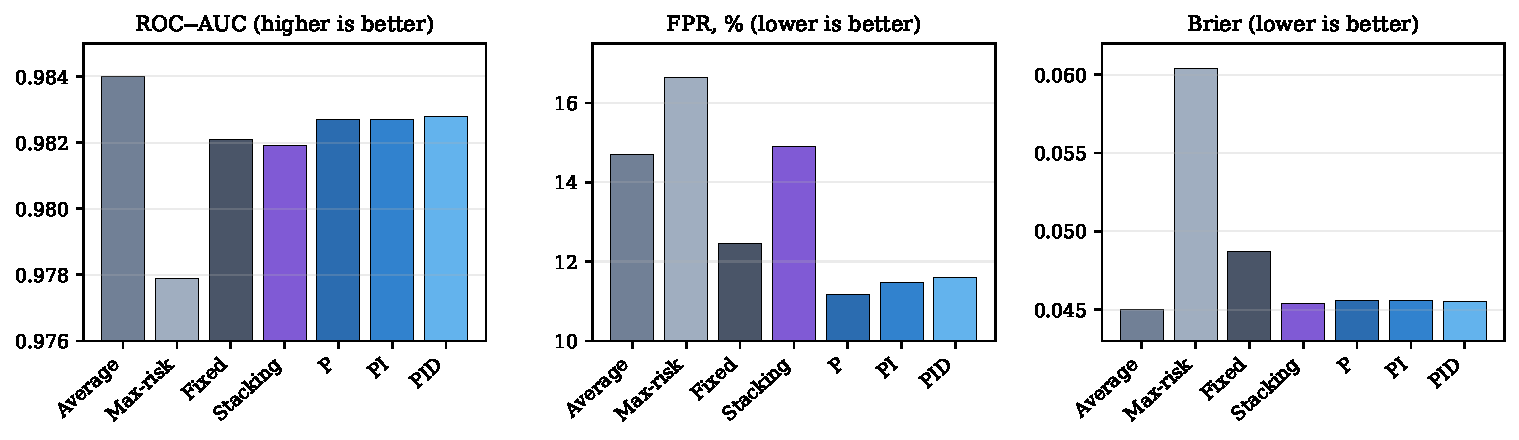
\includegraphics[width=0.94\textwidth]{fusion_summary.pdf}
\caption{Fusion discrimination, false-positive rate, and Brier score on the
paired development cohort. Values are aggregate means supplied by the retained
report; error bars are omitted because method-level fold vectors are not present
in this writing checkout.}
\label{fig:fusion-summary}
\end{figure*}

\subsubsection{Paired effects and controller ablation}

Table~\ref{tab:fusion-effects} reports the paired comparisons that govern the
claim. Adaptive P reduces FPR by 1.28 percentage points relative to Fixed, with
95\% CI $[-2.47,-0.11]$. It also reduces Brier by 0.00306, with CI
$[-0.00585,-0.00030]$. The TPR difference is $-0.10$ percentage point and its
interval crosses zero. In counts, P produces 104 false positives versus 116 for
Fixed and 950 true positives versus 951. The supported statement is improved FPR
and calibration with no detected material TPR loss on this development cohort.

\begin{table*}[t]
\centering
\caption{Primary paired fusion effects. Percentage-point (pp) effects are method
minus comparator. The two methods in a row can use independently validation-
selected thresholds.}
\label{tab:fusion-effects}
\small
\setlength{\tabcolsep}{3.5pt}
\begin{tabular}{p{3.1cm}p{2.6cm}p{2.1cm}p{3.0cm}p{4.0cm}}
\toprule
Comparison & Metric & Difference & 95\% CI & Interpretation \\
\midrule
Adaptive P $-$ Fixed & FPR & $-1.28$ pp & $[-2.47,-0.11]$ & Lower observed false-positive rate \\
Adaptive P $-$ Fixed & Brier & $-0.00306$ & $[-0.00585,-0.00030]$ & Lower squared probability error \\
Adaptive P $-$ Fixed & TPR & $-0.10$ pp & includes 0 & No detected TPR difference \\
Full PID $-$ Stacking & FPR & $-3.32$ pp & $[-4.94,-1.72]$ & Lower FPR at separately selected operating point \\
Full PID $-$ Stacking & AUC & $+0.08$ pp & $[-0.19,+0.37]$ & Comparable ranking; interval includes 0 \\
Full PID $-$ Stacking & TPR & $-0.62$ pp & $[-1.21,0.00]$ & Small sensitivity trade-off \\
Full PID $-$ Adaptive P & FPR & $+0.43$ pp & $[+0.11,+0.86]$ & I/D worsen FPR relative to P \\
\bottomrule
\end{tabular}
\end{table*}

Full PID versus Logistic stacking illustrates a different trade-off. PID lowers
FPR by 3.32 percentage points, but the thresholds are selected independently and
TPR is 0.62 percentage point lower. Its AUC difference is only $+0.08$
percentage point with an interval spanning zero. We therefore describe AUC as
comparable and avoid a same-TPR or universal-superiority claim.

The nested comparison is decisive for controller complexity. Full PID increases
FPR by 0.43 percentage point over Adaptive P while TPR is unchanged. The original
confirmatory ablation reached the same qualitative conclusion: turning off
$K_d$ while retaining $K_p,K_i$ changed none of the 1,922 final decisions, and D
altered only 6 of 7,688 intermediate-prefix decisions before the differences
disappeared at the final prefix. PID minus PI AUC was $-0.000125$ with an
interval crossing zero. Thus the retained event horizon does not support a
derivative benefit, and the integral term also fails to improve on P.

\subsubsection{Answer to RQ1}

Current static--dynamic disagreement can usefully adapt the mixture: Adaptive P
improves FPR and Brier over Fixed on the measured development cohort. Full PID
can achieve AUC comparable to learned stacking and a lower FPR at its own
selected operating point, with a small TPR trade-off. The available evidence
does not support incremental I/D complexity, closed-loop stability, sleep-
evasion handling, wall-clock latency reduction, or external validation.

\subsection{RQ2: Explanation-Guided Label Allocation}

\subsubsection{Learning-curve quality and target attainment}

Table~\ref{tab:al-main} integrates performance across 200--1,200 training labels.
$U+H$ achieves the highest ROC-AULC (0.933026) and AP-AULC (0.883336). Relative
to Random, its paired fold improvements are +0.004249 ROC-AULC and +0.014985
AP-AULC in the favorable direction in all five folds. Gains over Uncertainty are
smaller: +0.001754 and +0.001401, favorable in four of five folds.

\begin{table*}[t]
\centering
\caption{Confirmatory active-learning performance, target attainment, and
computation. Labels-to-target excludes validation labels and full-pool reference
cost.}
\label{tab:al-main}
\small
\setlength{\tabcolsep}{5pt}
\begin{tabular}{lccccc}
\toprule
Policy & ROC-AULC & AP-AULC & Labels to target & Query, 10 rounds (s) & Model + query (s) \\
\midrule
Random & 0.928777 & 0.868350 & 584 & 0.0194 & 4.1947 \\
Uncertainty & 0.931272 & 0.881934 & 520 & 0.0191 & 4.1454 \\
$U+H$ & \textbf{0.933026} & \textbf{0.883336} & 508 & 0.2459 & 4.4741 \\
$U+V$ & 0.930377 & 0.880164 & \textbf{488} & 0.2298 & 4.3826 \\
\xfull & 0.932202 & 0.881638 & 492 & 0.2358 & 4.3471 \\
\bottomrule
\end{tabular}
\end{table*}

$U+V$ reaches the validation target with the fewest mean training labels (488),
while \xfull reaches it with 492. Relative to Random's 584, \xfull reduces
the mean training budget by 92 labels, or 15.8\%. It also uses 28 fewer labels
than Uncertainty, but this advantage does not imply consistent superiority in
learning-curve ranking. Figure~\ref{fig:al-summary} shows that each
explanation-guided policy emphasizes a different criterion.

\begin{figure*}[t]
\centering
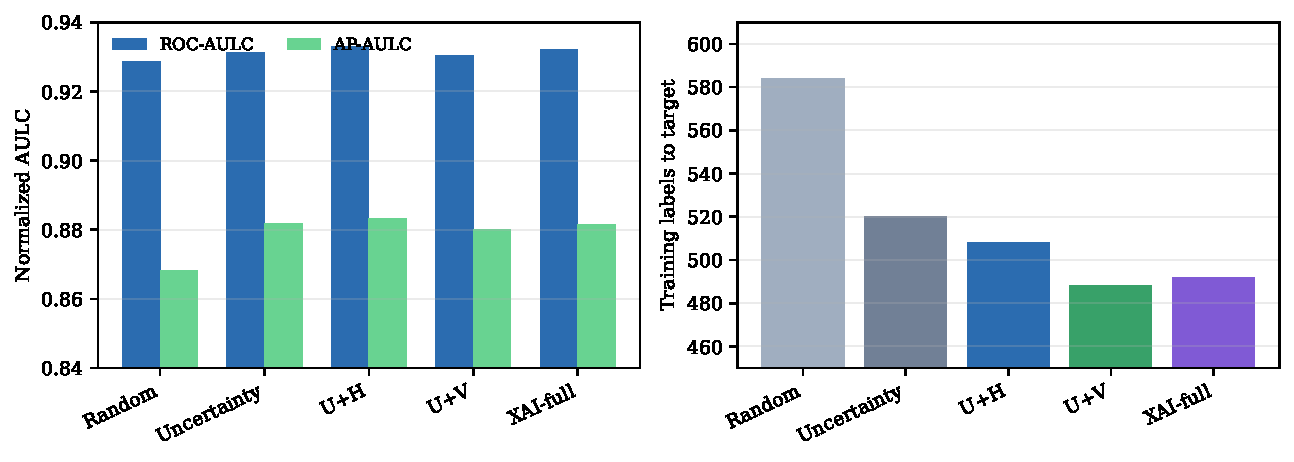
\includegraphics[width=0.93\textwidth]{al_summary.pdf}
\caption{Confirmatory active-learning summaries. Higher AULC is better; fewer
training labels to the predeclared validation target are better. Error bars are
omitted because the source-of-truth report provides aggregate means and paired
effects rather than fold vectors in this checkout.}
\label{fig:al-summary}
\end{figure*}

\begin{table}[t]
\centering
\caption{Selected paired outer-fold AL effects.}
\label{tab:al-effects}
\scriptsize
\setlength{\tabcolsep}{1pt}
\begin{tabular}{@{}lrrc@{}}
\toprule
Comparison & $\Delta$ROC & $\Delta$AP & Favorable folds \\
\midrule
$U+H$ vs. Random & +0.004249 & +0.014985 & 5/5 \\
$U+H$ vs. Uncertainty & +0.001754 & +0.001401 & 4/5 \\
\xfull vs. Random & +0.003425 & +0.013287 & 5/5 \\
\xfull vs. Uncertainty & +0.000931 & $-0.000297$ & 3/5 ROC \\
\bottomrule
\end{tabular}
\end{table}

Table~\ref{tab:al-effects} limits the strongest claim. \xfull improves over
Random in both AULC metrics and all five fold directions, but its AP-AULC
difference from Uncertainty is slightly negative and its ROC improvement occurs
in only three of five folds. Directional entropy provides the most consistent
measured addition; the three-signal policy is not a universal winner.

\subsubsection{Restricted-FPR behavior and computation}

Table~\ref{tab:low-fpr} shows that Uncertainty remains strong in restricted-FPR
regions. It leads normalized partial AUC at FPR$\leq5\%$ and TPR-AULC at the 1\%
cap; \xfull leads only at the 5\% cap. Explanation-guided policies clearly
improve over Random, but their differences from Uncertainty are small and metric
dependent. Each outer test fold contains roughly 300 benign rows, so a single
false positive changes FPR by about 0.33 percentage point. The data cannot
resolve production regions several orders of magnitude lower.

\begin{table*}[t]
\centering
\caption{Active-learning summaries in restricted false-positive regions.}
\label{tab:low-fpr}
\small
\begin{tabular}{lccc}
\toprule
Policy & pAUC, FPR$\leq5\%$ & TPR-AULC, FPR cap 1\% & TPR-AULC, FPR cap 5\% \\
\midrule
Random & 0.804096 & 0.580620 & 0.731980 \\
Uncertainty & \textbf{0.826300} & \textbf{0.638180} & 0.769260 \\
$U+H$ & 0.824774 & 0.636780 & 0.770620 \\
$U+V$ & 0.825194 & 0.626260 & 0.768140 \\
\xfull & 0.823525 & 0.631860 & \textbf{0.771460} \\
\bottomrule
\end{tabular}
\end{table*}

$U+H$ increases total model-plus-query time by about 7.93\% relative to
Uncertainty. \xfull increases it by 4.86\%, and query computation accounts
for approximately 5.42\% of its reported model-plus-query time. These small
absolute times apply to a 2,000-row experiment and omit analyst annotation and
production feature extraction.

\subsubsection{Answer to RQ2}

Explanation-derived signals add useful information relative to random
acquisition. Directional entropy yields the strongest integrated learning
trajectory; variance reaches the declared target with the fewest labels; and the
full policy saves 92 training labels relative to Random. Improvements over
uncertainty alone are smaller and change with the metric. The evidence supports
objective-dependent sample prioritization, not a single dominant policy or a
measured reduction in analyst hours.

\subsection{RQ3: Quantitative TreeSHAP Validation}

\subsubsection{Controlled deletion}

Table~\ref{tab:deletion} reports AUC decreases over 25 fitted models. Top-
$|\mathrm{SHAP}|$ deletion has a large monotonic effect as $k$ increases, whereas
uniform random deletion remains near zero. Under mean replacement at $k=50$,
the decreases are 0.306729 and 0.000979, an absolute difference of 0.305750.
Median replacement gives a similar difference of 0.300119. The conclusion is
robust to the two training-derived replacement baselines.

\begin{table*}[t]
\centering
\caption{Controlled feature-space deletion. Values are ROC--AUC decreases from
the corresponding unmasked model.}
\label{tab:deletion}
\small
\begin{tabular}{lrrrr}
\toprule
Replacement & $k$ & Top-SHAP drop & Random drop & Top minus random \\
\midrule
Mean & 10 & 0.047817 & 0.000200 & 0.047617 \\
Mean & 25 & 0.135853 & 0.000530 & 0.135323 \\
Mean & 50 & \textbf{0.306729} & 0.000979 & \textbf{0.305750} \\
Median & 10 & 0.053483 & 0.000094 & 0.053388 \\
Median & 25 & 0.125180 & 0.000326 & 0.124854 \\
Median & 50 & \textbf{0.300777} & 0.000658 & \textbf{0.300119} \\
\bottomrule
\end{tabular}
\end{table*}

\begin{figure}[t]
\centering
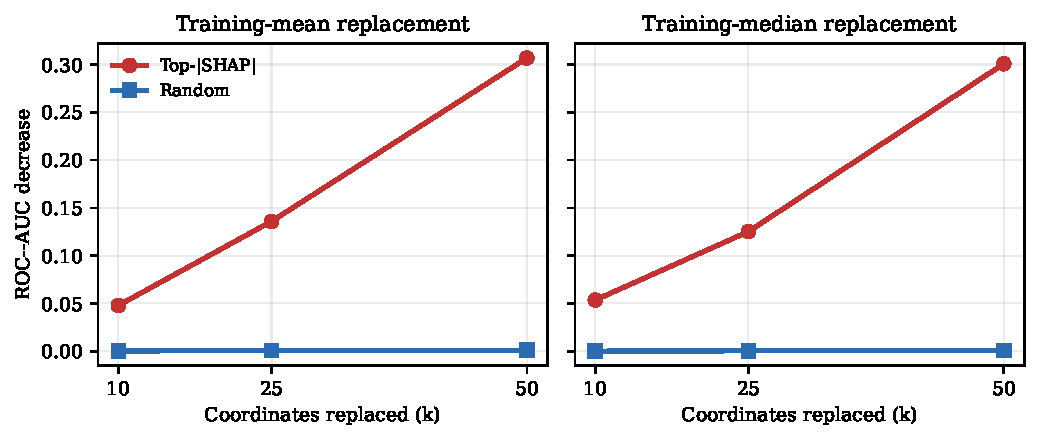
\includegraphics[width=\linewidth]{fidelity_deletion_confirmatory.pdf}
\caption{AUC decrease under top-$|\mathrm{SHAP}|$ and equal-count random
replacement. Absolute effects are emphasized because a ratio is unstable when
the random-control decrease is near zero.}
\label{fig:deletion}
\end{figure}

Equal coordinate count is an incomplete control. Uniform masks often select
inactive tree features and do not match standardized displacement or manifold
distance. The result nevertheless demonstrates relative fitted-model reliance:
under both specified interventions, TreeSHAP ranks coordinates whose replacement
changes ranking much more than uniformly chosen coordinates. It does not show a
valid edit to a PE file or a causal malware mechanism.

\subsubsection{Rank stability}

Within a fixed fold, global Spearman agreement is 0.6144, and top-10 Jaccard
agreement is 0.6221. Across folds, Spearman falls to 0.5512 and top-10 Jaccard to
0.4416. Agreement decreases further at larger top sets across folds. The ranking
is therefore neither arbitrary nor invariant; the training partition changes it
more than controlled model randomness.

\begin{table}[t]
\centering
\caption{TreeSHAP ranking stability.}
\label{tab:stability}
\scriptsize
\begin{tabular}{lrrrr}
\toprule
Comparison & $\rho$ & $J_{10}$ & $J_{25}$ & $J_{50}$ \\
\midrule
Seed, same fold & 0.6144 & 0.6221 & 0.5398 & 0.4901 \\
Different fold & 0.5512 & 0.4416 & 0.3073 & 0.3020 \\
\bottomrule
\end{tabular}
\end{table}

\begin{figure}[t]
\centering
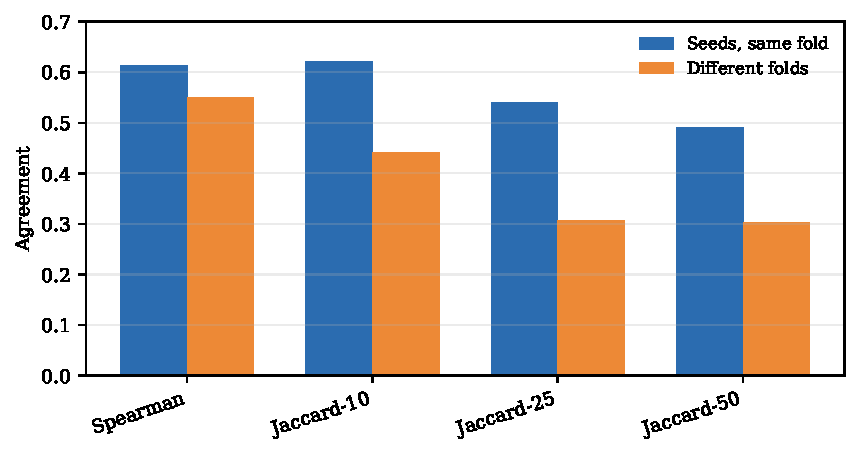
\includegraphics[width=\linewidth]{shap_stability_confirmatory.pdf}
\caption{Global and top-$k$ attribution agreement. Fold changes have a larger
effect than seed changes within the same fold.}
\label{fig:stability}
\end{figure}

Mean EC is $0.4268\pm0.0363$ and mean CF is $0.4680\pm0.0465$ across 25 models.
Maximum additivity error is approximately $6\times10^{-15}$. These values
describe geometry and numerical consistency; they are not combined into a
fidelity certificate.

\subsubsection{Answer to RQ3}

TreeSHAP top-ranked coordinates exert substantially greater model-ranking impact
than equal-budget random coordinates under both mean and median replacement.
Moderate stability supports repeatable model reliance while exposing meaningful
partition sensitivity. The evidence is quantitative but model relative: it does
not establish feature causality, executable-valid masking, or timeless malware
semantics.

\subsection{Exploratory Fusion Extensions}

The 1,186-sample horizon-40 subset was used after observing the horizon-20
limitations and is therefore exploratory. Robust PID v2 reached AUC 0.9895 and
AP 0.9911, equal at reported precision to Logistic stacking, with FPR 3.35\%
versus 3.68\% and TPR 94.32\% versus 94.84\%. The AUC difference interval
$[-0.0008,+0.0008]$ and FPR interval both include zero. Against the older PID
full v2, Robust PID v2 reduces FPR by 1.33 percentage points with CI
$[-2.66,-0.15]$. This supports an algorithm candidate, not independent
confirmation.

A gated residual PID stress test under a controlled five-event delay reports FPR
2.61\% versus 3.93\% for Temporal stacking and TPR 94.49\% versus 94.66\%.
It removes eight false positives, creates none, and loses one true positive;
Holm-adjusted $p=0.0312$. Three of five folds select zero gain, and event-AULC
does not improve. This evidence is limited to the specified stress construction.

Finally, the timestamp pilot downloads reports for 20 selected samples and finds
eight usable event sequences with 4,697 API--timestamp pairs. It demonstrates
that wall-clock sequences can be parsed. With only two usable benign and six
malware sequences, it cannot evaluate performance, latency, or the derivative
term. These exploratory results define the next confirmatory experiment and do
not change the main RQ1 conclusion.

\section{Discussion}
\label{sec:discussion}

\subsection{A Unified Flow without an Integrated Claim}

The three components address one recurring security-learning problem: useful
evidence is incomplete, arrives at different times, and has different costs.
Static and dynamic scores allocate evidence to an online decision. Active
learning allocates a label budget to model maintenance. TreeSHAP diagnostics
allocate confidence to an explanation ranking used in that maintenance process.
This flow is scientifically useful because it identifies the interfaces a future
system must validate: paired channel identity, acquisition lineage, and
explanation checks.

The flow is not itself an empirical interaction. MalBehavD-V1 does not contain
the EMBER active-learning artifact, and EMBER does not contain the ordered
dynamic observation required for fusion. Consequently, the study cannot answer
whether explanation-guided retraining improves the fused detector, whether PID
changes which samples should be queried, or whether one common threshold reduces
end-to-end alert cost. A factorial experiment on one paired cohort remains
necessary. Preserving this boundary makes the component results easier to audit
and prevents a conceptual architecture from becoming a fabricated system score.

\subsection{What the PID Translation Establishes}

The control analogy provides a disciplined set of nested hypotheses. P asks
whether current detector disagreement should alter the mixture. I asks whether
persistent signed disagreement supplies additional information. D asks whether a
change in disagreement across event prefixes predicts useful adjustment. The
empirical result supports the first hypothesis and rejects the need for the
latter two under the measured horizon.

This outcome is plausible. The static score is constant within a sequence, while
the dynamic score updates at short API prefixes. If successive prefixes change
only a few events, the derivative term can be sparse or noisy. If one channel is
systematically higher for a source, the integral may accumulate collection bias
rather than sample-specific reliability. A proportional mapping can capture the
dominant behavior with fewer states and lower implementation risk. Adaptive P's
FPR and Brier improvements over Fixed make it a stronger current candidate than
full PID for horizon 1--20.

The result also clarifies what PID cannot do. It cannot reveal behavior that the
sandbox never observes. It cannot turn event count into elapsed time. It cannot
guarantee calibration or stability from control theory alone. Sleep-evasion
resistance would require real timestamped traces, controlled delayed behavior,
and a specified observation policy. End-to-end latency would require separate
measurement of queueing, sandbox startup, observation, feature extraction,
channel inference, and fusion. The small timestamp pilot begins data-source
validation but does not satisfy those requirements.

Learned stacking remains an important baseline. Full PID has comparable AUC and
lower FPR at its own operating point, but also a small TPR reduction. Average has
the best Brier and slightly higher AUC than the adaptive family. These results
show that interpretability and operating-point objectives, rather than a tiny
AUC difference, must motivate an adaptive controller. External validation at a
common target TPR should decide whether Adaptive P's lower FPR transfers.

\subsection{What the Acquisition Result Means}

Directional entropy adds a small and repeatable learning-curve improvement over
Random and a smaller improvement over Uncertainty in four of five folds. It
distinguishes two probability-equivalent cases: weak evidence and stronger
opposing signed masses. Such conflict can identify a model region where a new
label is useful. The algebra in Equation~(\ref{eq:h-identity}) narrows this
interpretation: $H$ is determined by the total raw-score contribution and the
$L_1$ attribution norm. A direct margin-plus-norm baseline may recover part of
the effect and should be included in an extension.

No acquisition policy dominates every objective. $U+H$ leads AULC, $U+V$
reaches the target earliest, \xfull balances signals and saves 92 labels
relative to Random, and Uncertainty remains strongest in two restricted-FPR
summaries. Policy selection should therefore follow the maintenance objective.
An organization prioritizing average model quality during iterative labeling may
prefer $U+H$; one using the retained validation target may prefer $U+V$; one
requiring low computation and strong low-FPR behavior may retain Uncertainty.

The label result has an explicit accounting boundary. It counts labels added to
training. Validation labels, initial dataset creation, the full-pool reference,
analyst abstention, and disagreement resolution remain outside the number. A
15.8\% label-count reduction is not a measured 15.8\% reduction in labor.

Batch redundancy is an unresolved alternative explanation. Selecting the top
100 pointwise scores can query many objects from one region. Uncertainty plus
k-center selection would test whether simple diversity reproduces the gain. A
calibrated committee would test whether ensemble disagreement explains the
benefit. Robust quantile or rank normalization would test sensitivity to extreme
$H$ or $V$ values that compress min--max scaling. These settings must be frozen
within a nested design, not chosen by outer-test AULC.

\subsection{What the TreeSHAP Audit Establishes}

Top-ranked replacement damages model ranking much more than uniform random
replacement under both training means and medians. This is strong evidence of
relative model reliance under the defined feature-space intervention. It is
particularly useful as an internal release check: a TreeSHAP ranking that fails
to exceed equal-count random deletion should not be presented as a meaningful
ordering of influential coordinates.

The deletion gap is not a causal certificate. Tree ensembles use a subset of
2,381 coordinates, so random masks often strike inactive features. Top-ranked
coordinates may also be farther from the replacement baseline, creating a larger
standardized displacement and greater off-manifold shift. Stronger controls
should sample only used features, match displacement magnitude, replace
semantically linked PE groups, and use conditional backgrounds. Reconstructing
valid PE binaries would answer a different and substantially harder question.

Moderate stability gives a complementary warning. Explanations change less
across model seeds in one fold than across folds, showing that data composition
matters. A global top-feature list should therefore be versioned with the model,
feature schema, and training cohort. For active learning, round-specific change
is expected because the model is retrained, but abrupt attribution drift should
be logged and investigated.

Additivity, EC, and CF remain diagnostics of numerical or geometric properties.
A common permutation of attribution columns can preserve sums, cosines, norms,
and centroid separation while giving effects the wrong feature identities.
Combining such heterogeneous quantities into an unvalidated Overall Fidelity
Score would hide this weakness. Separate reporting is more informative and more
defensible.

\subsection{Operational Interpretation}

The most immediate use is a controlled model-development workflow. A candidate
static model scores a pool; a chosen acquisition rule prioritizes objects for an
authorized analyst; query/model lineage is retained; and deletion/stability
checks are run before release. Separately, when a paired dynamic sequence is
available, Adaptive P can be compared against Average, Fixed, and Stacking at a
locked operating objective. The evidence does not yet authorize automated
remediation or deployment claims.

Scaling introduces additional costs. TreeSHAP over a large candidate pool can be
reduced by first filtering a probability band, but that changes the acquisition
population and requires reevaluation. Dynamic collection dominates arithmetic
fusion cost, so optimizing the PID calculation alone will not solve system
latency. These practical distinctions follow directly from the unified evidence-
allocation view: computation, labels, observation time, and alert errors are
different resources and should be measured separately.

\subsection{Evidence Needed for a Stronger Journal Claim}

The highest-priority experiment is an external or temporal paired cohort whose
method and thresholds are frozen before access. Adaptive P and robust PID v2
should be preregistered with a common-TPR comparison and noninferiority or
superiority margins. Timestamped event sequences should support separate early-
detection and wall-clock analyses. The same cohort should then receive a
factorial acquisition--fusion evaluation if interaction is claimed.

For RQ2/RQ3, the strongest additions are uncertainty plus diversity, a calibrated
committee, weight/normalization sensitivity, family- or time-aware splits,
used-feature and magnitude-matched deletion controls, conditional/group masking,
and a second explainer. These experiments address plausible alternatives to the
current effects and determine how far they generalize beyond the audited subset.

\section{Threats to Validity}
\label{sec:threats}

\subsection{Construct Validity}

Both datasets encode generic benign/malware labels. Neither establishes
ransomware membership, ransomware behavior, or zero-day status. AVClass metadata
is incomplete and not used as behavioral ground truth. The paper therefore uses
the term Windows malware and treats ransomware-specific detection as future
work.

MalBehavD-V1 prefixes are ordered by API-event count. Event 20 is not 20 seconds,
and a lower arithmetic fusion cost does not imply earlier wall-clock detection.
Detector disagreement is a surrogate fusion signal, not the tracking error of a
physical plant. Terms such as proportional, integral, and derivative describe
the mathematical update only; they do not confer closed-loop stability.

Directional entropy is entropy of positive/negative attribution mass, not
predictive class entropy. Attribution variance is dispersion across coordinates
of one SHAP vector, not epistemic variance. “Explanation-guided” describes the
source of the acquisition signals, not proof that they encode human-understandable
malware mechanisms.

Deletion measures fitted-model behavior under feature replacement. It does not
establish causal features, valid PE transformations, adversarial robustness, or
analyst usefulness. EC, CF, and additivity measure different constructs and are
not aggregated into an Overall Fidelity Score.

\subsection{Internal Validity}

Fusion methods use paired static/dynamic rows and validation-selected settings,
which reduces channel and threshold confounding. Yet the adaptive fusion design
was developed after inspecting the original confirmatory result on the same
1,922-sample cohort. The resulting test-row estimates are development evidence;
same-cohort bootstrap intervals cannot remove method-selection bias. Source
differences between benign and malware data may also influence both channel
scores despite exclusion of explicit verdict and threat-name metadata.

For AL, outer test partitions do not enter query selection or target definition,
and policies share initial sets within a fold/seed. The fixed acquisition weights
and min--max normalization were not selected through an independent outer
sensitivity analysis. Pointwise top-100 selection has no diversity constraint.
The simulated oracle returns retained labels without error, whereas analysts can
abstain, disagree, or use different evidence.

For fidelity, mean and median baselines use training data, avoiding direct test
leakage. Top and random masks are matched by coordinate count but not by
standardized displacement, tree usage, semantic group, or manifold distance.
These differences can inflate the top-minus-random gap. Masked test vectors are
not verified against the PE format.

\subsection{Statistical Conclusion Validity}

Fusion confidence intervals are paired over retained predictions, but only one
development cohort is available. Multiple metrics and method comparisons create
selection opportunities, and no external confirmatory family controls them. FPR
and TPR use validation-selected operating points; the PID--stacking FPR
difference is not a comparison at equal TPR.

The AL comparison unit is the outer fold after averaging five seed trajectories.
Five folds provide effect sizes and direction counts but limited asymptotic
inference. Twenty-five fold--seed runs do not represent 25 independent datasets.
The source report supplies aggregate values and selected paired effects rather
than fold vectors in this checkout, so reconstructed figures omit uncertainty
bars.

Restricted-FPR estimates use small test folds. With approximately 300 benign
rows, one false positive changes FPR by roughly 0.33 percentage point. Results at
1\% or 5\% caps cannot validate alert rates at $10^{-3}$ or $10^{-4}$.

The 25 fidelity models share folds and data; they are not independent population
draws. Random masks characterize conditional mask variability. Pairwise
stability values share fitted models and cannot be entered as independent rows
in a naive significance test.

\subsection{External Validity}

The 2,000-row EMBER subset covers a short 2018 period and uses random row folds.
It does not impose temporal, family, campaign, or source separation. The
MalBehavD-V1 cohort is also one source with metadata-availability and minimum-
event selection. Results can change for newer software, different organizations,
other sandbox environments, or another feature extractor.

The horizon-40 subset was selected after horizon-20 results were known. Robust
PID v2 and controlled stress findings are therefore explicitly exploratory. The
timestamp pilot contains only eight usable sequences and cannot support
performance inference. No measured result covers production queueing, analyst
workflow, or end-to-end incident response.

LightGBM and TreeSHAP are central to RQ2/RQ3. The acquisition summaries can be
defined for other additive attributions, but their numeric behavior, cost, and
stability may differ for raw-byte networks, graph models, or sequence models.

\subsection{Integration Validity}

The three RQs use two datasets and different feature spaces. The architecture
connects them as stages of an auditable learning process, but the experiments do
not demonstrate a single deployed pipeline. There is no measured gate deciding
which EMBER sample receives dynamic analysis, no AL retraining of the
MalBehavD-V1 fusion channels, and no shared latency/cost objective. Claims about
synergy, interaction, or complete-system superiority are outside the evidence.

\subsection{Reproducibility Validity}

The source-of-truth report names commit \texttt{8bfa06b65b93}, dataset hashes,
result directories, and verification artifacts. The remote branch available in
the writing environment ends at an older commit, so the manuscript was generated
from the supplied report rather than by rerunning the missing artifacts. Tables
and plots reproduce reported aggregate values; they do not constitute an
independent computational replication.

Before submission, the named commit and all result directories must be pushed,
hashes checked, verification commands rerun in a clean environment, and tables
and figures regenerated directly from fold-level records. Bibliographic metadata,
data-sharing rights, authorship order, corresponding author, and the target
journal template also require final verification. Computational replay can show
consistency with stored code and data; it cannot prove upstream label accuracy or
external generalization.

\section{Conclusion}
\label{sec:conclusion}

This paper formulated Windows malware model development as auditable evidence
allocation under partial observability. The decision stage combines early static
evidence with event-indexed dynamic evidence; the adaptation stage assigns a
limited labeling budget; and the audit stage tests the attribution ranking used
in model inspection and acquisition. The formulation provides one scientific
flow while preserving component-specific estimands and datasets.

On the 1,922-sample MalBehavD-V1 development cohort, Adaptive P reduced FPR from
12.45\% to 11.16\% relative to fixed weighting and reduced Brier by 0.00306,
with paired intervals excluding zero. Full PID obtained AUC comparable to
logistic stacking and a lower FPR at its independently selected operating point,
with a small TPR trade-off. Integral and derivative terms did not add consistent
value over P within 1--20 event prefixes. The evidence therefore favors a
simpler proportional adaptation and treats richer PID variants as hypotheses for
external timestamped evaluation.

On the identity-audited 2,000-sample EMBER subset, $U+H$ produced the strongest
ROC/AP learning-curve areas. $U+V$ reached the predeclared target with the fewest
labels, while \xfull used 492 labels, 92 fewer than Random. Gains over
Uncertainty were smaller and metric dependent. Across 25 fitted models,
top-$|\mathrm{SHAP}|$ deletion produced much larger AUC decreases than equal-
budget random deletion under mean and median replacement, while moderate
stability revealed dependence on data partitions.

These results support component-wise adaptive fusion, explanation-guided sample
prioritization, and quantitative attribution auditing for generic Windows
malware. They do not establish ransomware detection, causal PE explanations,
external generalization, or an end-to-end integrated system. The next evidence
gate is a frozen external or temporal paired cohort with common operating targets
and real timestamps, followed by stronger AL diversity baselines, conditional
deletion controls, and a factorial acquisition--fusion experiment on one cohort.


\appendices
\section{Fusion Replay and External-Validation Checklist}
\label{app:fusion}

A submission-quality replay of RQ1 should retain, for every outer fold:

\begin{enumerate}
    \item the cohort manifest with SHA-256, label, split, session/sequence ID,
    static metadata row, and ordered dynamic event identifiers;
    \item proof that verdict, detection-count, threat-name, filename, and other
    direct label proxies are excluded from the static allow-list;
    \item channel models, calibration objects, prefix scores, validation/test
    predictions, and the provenance of each score;
    \item fixed-weight grid, stacking configuration, P/PI/PID settings,
    controller-state reset, clipping rule, and deterministic tie breaking;
    \item validation-only selection records for gains, mixture settings, and
    thresholds, with no state transfer into held-out rows;
    \item per-prefix and final predictions for Average, Max-risk, Fixed,
    Stacking, P, PI, and PID using identical paired inputs;
    \item ROC--AUC, AP, Brier, FPR, TPR, confusion counts, and paired bootstrap
    indices sufficient to reproduce every interval;
    \item separate wall-clock measurements for collection, feature extraction,
    channel inference, fusion arithmetic, queueing, and total response if a
    latency claim is introduced.
\end{enumerate}

The external experiment should freeze Adaptive P and any robust PID candidate
before data access. A common target TPR or a preregistered cost function should
govern threshold comparison. Noninferiority and superiority margins must be
declared before evaluation. Timestamped sequences should establish whether a
derivative term sees meaningful elapsed-time change rather than event-count
noise.

\section{Active-Learning Replay Checklist}
\label{app:al}

For each outer fold and AL seed, retain:

\begin{enumerate}
    \item development, validation, and test row identifiers;
    \item the shared 200-row initial labeled set and ordered remaining pool;
    \item model configuration, library versions, and deterministic seeds;
    \item validation/test probabilities and labels at every round;
    \item pool probabilities, $U/H/V$ components, normalized values, composite
    scores, ranks, and queried row identifiers;
    \item the full-pool validation reference and target calculation;
    \item per-round ROC--AUC, AP, low-FPR summaries, and scoped timing records;
    \item checkpoints or a deterministic reconstruction mechanism;
    \item verification of query membership, uniqueness, additivity, metric
    recomputation, and absence of validation/test leakage.
\end{enumerate}

Every policy in a fold/seed must begin from the same initial set. The test
partition must remain unavailable to query selection, target construction,
threshold choice, weight selection, and stopping. A stronger extension should
add uncertainty plus k-center diversity, a calibrated committee, direct
margin-plus-attribution-norm controls, and frozen sensitivity grids for
normalization and $\alpha,\beta,\gamma$.

\section{TreeSHAP Audit Checklist}
\label{app:fidelity}

For each fold and model seed:

\begin{enumerate}
    \item retain the fitted model, split IDs, feature schema, training mean and
    median, and raw TreeSHAP matrix with bias stored separately;
    \item verify raw-score additivity before ranking features;
    \item save top-$k$ and random mask indices for every sample, $k$, control
    draw, and replacement baseline;
    \item reconstruct masked matrices from original test vectors and saved
    indices, rather than from plotted summaries;
    \item retain original and masked probabilities and recompute AUC decreases;
    \item retain global rankings and model-pair identifiers used for Spearman and
    Jaccard summaries;
    \item label EC/CF as geometry diagnostics and confirm that no composite OFS
    is introduced without validated scaling, weights, and sensitivity analysis.
\end{enumerate}

Required stronger controls include random masks restricted to model-used
features, standardized-displacement matching, attribution-column permutation,
schema-aware group replacement, conditional backgrounds, and comparison with at
least one alternative explainer or importance method.

\section{Metric and Interpretation Boundaries}

\begin{table*}[h]
\centering
\caption{What the reported quantities establish and do not establish.}
\label{tab:boundaries}
\scriptsize
\setlength{\tabcolsep}{3pt}
\begin{tabular}{p{2.7cm}p{5.6cm}p{6.4cm}}
\toprule
Quantity & Supported interpretation & Unsupported interpretation \\
\midrule
Fusion AUC/AP & Ranking of paired cohort scores & Deployment utility or external transfer \\
FPR/TPR & Decisions at validation-selected thresholds & Same-TPR comparison when thresholds differ \\
Brier & Squared probabilistic error on the cohort & Complete calibration characterization \\
P improvement & Value of current disagreement in measured development cohort & Classical-control stability or universal PID value \\
I/D ablation & No stable incremental benefit in tested prefixes & Proof that temporal memory can never help \\
ROC/AP-AULC & Ranking quality integrated over measured label budgets & Analyst labor, calibration, or external generalization \\
Labels to target & Training labels to a fold-specific validation target & Total annotation cost or hours saved \\
Low-FPR AL summaries & Relative behavior at 1\%/5\% caps in outer folds & Reliable FPR at $10^{-3}$ or $10^{-4}$ \\
$H$ & Balance of positive/negative TreeSHAP mass & Predictive entropy or causal conflict \\
$V$ & Dispersion across signed attribution coordinates & Ensemble or posterior uncertainty \\
Top-$k$ deletion & Fitted-model sensitivity under training-statistic replacement & Valid PE transformation or causal malware mechanism \\
Additivity & Numerical reconstruction of the raw tree score & Correct feature identity or human usefulness \\
Seed/fold agreement & Sensitivity to fitted model and data partition & Stability across organizations and time \\
Replay verification & Consistency with retained code/data/artifacts & Independent replication or upstream data authenticity \\
\bottomrule
\end{tabular}
\end{table*}

\section{Claim--Evidence Map}

\begin{table*}[h]
\centering
\caption{Central claims, evidence tier, and manuscript status.}
\label{tab:claims}
\scriptsize
\begin{tabular}{p{5.2cm}p{3.1cm}p{6.8cm}}
\toprule
Claim & Status/tier & Required scope \\
\midrule
Adaptive P lowers FPR and Brier versus Fixed & Supported, development & 1,922-sample same-cohort development; paired intervals exclude zero \\
Full PID outperforms all fusion baselines & Not supported & Average leads AUC/Brier; P leads FPR; PID has TPR trade-off \\
I/D improve fusion & Not supported & No stable incremental benefit over P at 1--20 prefixes \\
Robust PID v2 matches stacking & Exploratory & Horizon-40 development subset; external confirmation pending \\
$U+H$ exceeds Random in ROC/AP-AULC & Supported, confirmatory & Five outer folds; paired effect and direction reported \\
$U+H$ universally exceeds Uncertainty & Not supported & Small effects; favorable in four of five folds \\
\xfull saves 92 training labels versus Random & Supported, confirmatory & Validation/reference and analyst cost are additional \\
\xfull is best on every criterion & Not supported & $U+H$ leads AULC; $U+V$ uses fewest labels \\
Top-SHAP deletion exceeds random deletion & Supported, confirmatory & Feature-space intervention; 25 models; mean/median \\
TreeSHAP identifies causal malware features & Not supported & No executable-valid or causal intervention \\
The complete architecture is validated end-to-end & Not supported & Two datasets and three component-level estimands \\
The study detects ransomware or zero-day malware & Not supported & Generic Windows malware labels only \\
\bottomrule
\end{tabular}
\end{table*}

\section{Artifact Traceability}

The submission package should map each paper object to the following retained
families:

\begin{itemize}
    \item \textbf{EMBER identity:}
    \path{results/confirmatory_20261019_ember_identity/}
    \path{static_identity_audit.json} and \path{SHA256SUMS}.
    \item \textbf{Active learning:} \path{al/aulc_summary.csv},
    \path{target_reach_summary.csv},
    \path{fold_level_effects.csv},
    \path{low_fpr_aulc_by_fold.csv},
    \path{overhead_by_fold.csv}, and \path{verification.json}.
    \item \textbf{Fidelity:} \path{fidelity/deletion_summary.csv},
    \path{shap_stability_summary.csv},
    \path{model_deletion_comparisons.csv}, and
    \path{verification.json}.
    \item \textbf{Fusion confirmatory:}
    \path{results/measured_20261023_malbehavd_pid_confirmatory_1922/}
    including cohort, source, summary, D-ablation, paired-bootstrap, and
    verification records.
    \item \textbf{Fusion development:}
    \path{results/measured_20261028_fusion_only_evidence_1922/}
    including \path{fusion_only_summary.json}.
    \item \textbf{Exploratory fusion:}
    \path{results/exploratory_20261028_pid_v2_meta_fusion_horizon40/}
    and the stateful/stress result families.
    \item \textbf{Timestamp feasibility:}
    \path{results/measured_20261028_vt_behaviour_pilot20/}.
\end{itemize}

The machine-readable companion file \path{CLAIM_EVIDENCE_MAP.csv} expands
this mapping with permitted manuscript locations and exact qualifiers.

\section{Pre-Submission Evidence Gates}

Before journal submission:

\begin{enumerate}
    \item synchronize source commit \texttt{8bfa06b65b93} and every artifact
    named above; run hash and replay verification in a clean environment;
    \item regenerate tables, confidence intervals, and figures directly from
    fold-level records, including uncertainty visualization;
    \item freeze Adaptive P/robust PID and run a new external or temporal cohort
    at a preregistered common operating target;
    \item add uncertainty-plus-diversity, a calibrated committee, and
    acquisition-weight/normalization sensitivity;
    \item add identity-sensitive, used-feature, magnitude-matched, and
    group-aware fidelity controls;
    \item obtain temporal, family-disjoint, or source-disjoint evidence if the
    target venue expects broad generalization;
    \item verify all bibliography metadata against publisher records and confirm
    authorship, ORCID, corresponding author, data rights, funding, conflicts, and
    the current journal template.
\end{enumerate}

\clearpage

\bibliographystyle{IEEEtran}
\bibliography{references}
\end{document}
